A Nacele é o compartimento situado no alto da torre e que comporta todos os componentes para a geração de energia responsável pela transformação de energia mecânica em energia elétrica. Seu tamanho e formato depende da presença de componentes e sua disposição em seu interior\cite{custodio2013}.Além dos componentes transformadores de energia, a nacele do projeto abrigará, também, todos os componentes envolvidos na obtenção da água pela umidade do ar. O desenvolvimento de materiais a serem utilizados devem ser destacados, uma vez que está relacionado diretamente com a produção de energia e com a redução de custos. A construção de turbinas eólicas devem ser preparadas para suportar diversas situações meteorológicas, existindo a necessidade de implantação de materiais mais leves e resistentes em todos os componentes. 	
	  
	As fibras de vidro pertencem a uma importante posição no mercado de materiais devido ao seu baixo coeficiente de dilatação térmica, facilidade de processamento, baixo custo e altas propriedades mecânicas e retenção desta em altas temperaturas3 e por isso escolhido para se construir a nacele.
	
	\begin{figure}[!htbp]
	 \centering
	  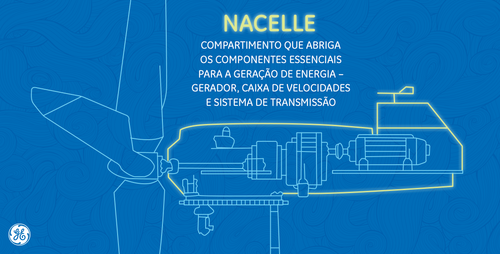
\includegraphics[scale=0.5]{editaveis/figuras/nacele}
	  \caption[nacele]{Nacele\footnotemark}
	  \label{nacele}
	\end{figure}
	\footnotetext{Disponível em: <http://www.tumblr.com/search/desenvolvemos\%20a\%20energia>}